\section{Statement of Problem}
Task 2 utilizes a wave ray tracing algorithm and local bathymetry information, provided for Narragansett Bay, in order to propagate storm waves determined from task 1. In order to complete this task, simulations are conducted for the 20 and 50 year storms along with creating rays that intersect along the shoreline of Narragansett Beach. For the 20 year storm simulations, use the ray spacing on the beach to calculate a refraction coefficient for each section of beach. Then, using bathymetry data from a chart near the beach, estimate the beach slope. This is used along with the deep water wave properties and refraction coefficient to estimate the shoaling coefficient, breaking depth, and breaker height. 
\section{Hypotheses and Theories}

When waves propagate over a non uniform sea floor, they refract depending on how the sea floor depth changes along the wavefront. As water depth decreases wave fronts can focus or de-focus along the coastline. Seen in \ref{eq:refrac_coeff}, the refraction coefficient can be determined with the distance between wave rays initially, and in the target location. A refraction coefficient less than one indicates de-focusing. 

\begin{equation}
K_{r} = \sqrt{\dfrac{b_{o}}{b}}
\label{eq:refrac_coeff}
\end{equation}

In shallow water, waves slow down and experience an increase in wave height due to shoaling. The degree of wave refraction, and the shoaling coefficient dictate breaking wave height and water depth. Seen in \ref{eq:shoaling_coeff}, the ratio of phase speed and group celerity changes as water depth approaches the shallow water condition. With the deep water characteristics, and angle of incidence, breaker depth and wave height can be found iteratively.

\begin{align}[H]
c = c_{o} * \tanh(kh); \\
c_{g} = \dfrac{c}{2} * \left(1 + \dfrac{2kh}{\sinh(2kh)}\right) \\
K_{s} = \sqrt{c/2c_{g}}
\label{eq:shoaling_coeff}
\end{align}

\begin{align}
H_{b} = H_{o}K_{sb}K_{rb} = \kappa h_{b}
\\ K_{sb} = F(L,h)
\\K_{rb} = F(L,h,\theta_{o})
\label{eq:breaker_char}
\end{align}

The programs supplied for the problem simulated waves propagating into the region of coastline surrounding Narragansett Beach. The programs required deep water wave characteristics, and latitude-longitude grid resolution. 

\section{Solution of the Problem}

Using the supplied C functions and waveray.m, wave rays were propagated into Narragansett Beach under the conditions determined in Task 1. Twenty and fifty year predicted wave parameters were used to simulate the path lines extreme waves followed. Seen in CITE WAVEDIR FIGURE HERE, three predominant angles of incidence were determined from the supplied data. Waveray.m  was non-intuitive, and didn't allow for significant manipulation of the rendered area without ruining the data. A consequence of this was that our breaking wave characteristics were evaluated manually, and were not based off the simulation data.

Seen below, the simulated wave rays from all three angles of incidence experienced de-focusing as they approached the beach. Significant focusing can be observed in \ref{fig20y210deg} further south on the shoreline. 

\begin{figure}[H]
\centering
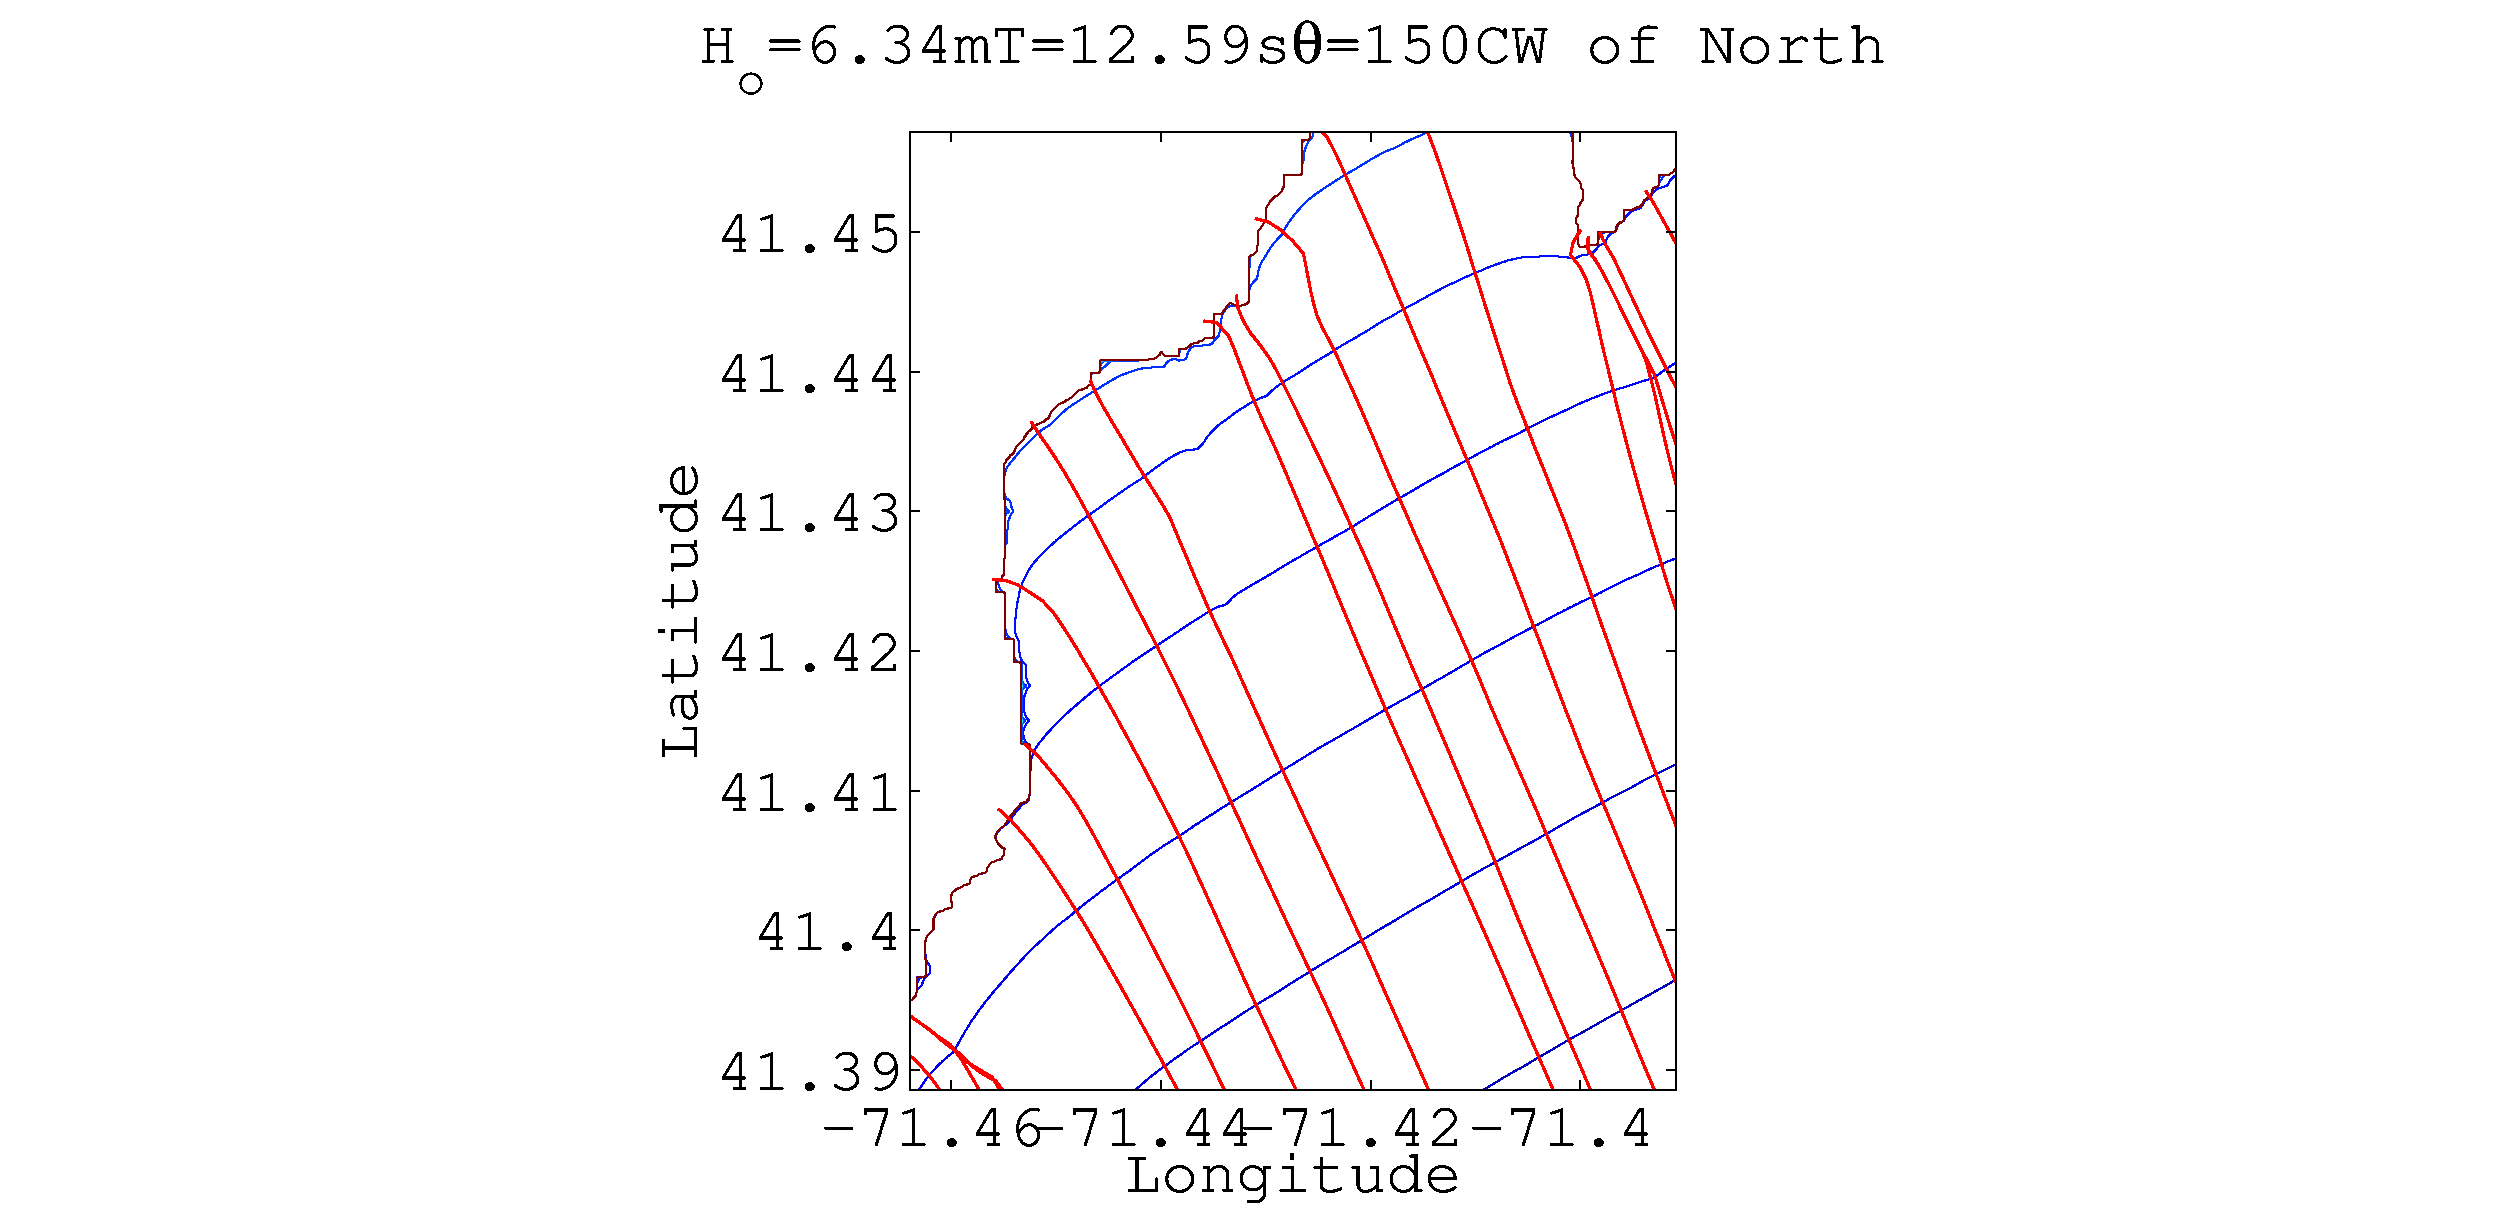
\includegraphics[width=1.0\textwidth]{./img/20y_150deg.pdf}
\caption{20y Predicted Wave Rays at 150$^{\circ}$ angle of incidence}
\label{fig:20y150deg}
\end{figure}

\begin{table}[H]
\centering
\begin{tabular}{ccccc}
$K_{r}$ & $K_{s}$ & $H_{b}$ & $h_{b}$ & $\dfrac{H_{b}}{h_{b}}$ \\
\hline
0.0 & 0.1 & 5.2 & 7.6 & 0.7 \\
1.0 & 0.0 & 3.4 & 7.5 & 0.5 \\
\hline
\end{tabular}

\caption{Breaking Wave Characteristics for 20 Year extreme wave at 180$^{\circ}$ angle of incidence}
\label{tab:20y_150deg}
\end{table}

\begin{figure}[H]
\centering
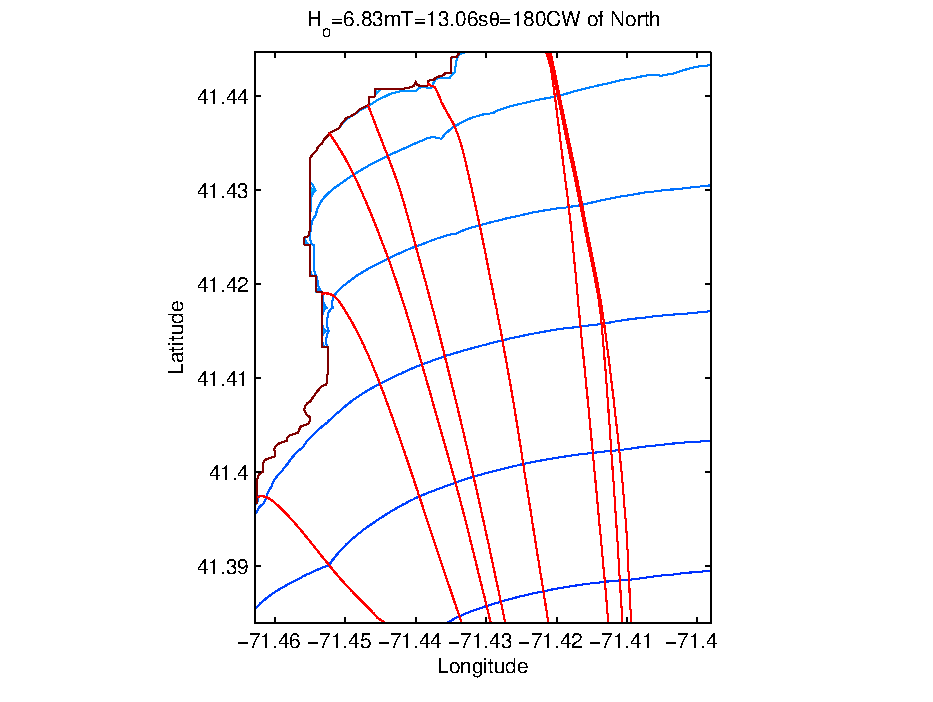
\includegraphics[width=0.6\textwidth]{./img/20y_180deg.pdf}
\caption{20y Predicted Wave Rays at 180$^{\circ}$ angle of incidence}
\label{fig:20y180deg}
\end{figure}

\begin{table}[H]
\centering
\begin{tabular}{cccccc}
Ray: & $K_{r}$ & $K_{s}$ & $H_{b}$ & $h_{b}$ & $\dfrac{H_{b}}{h_{b}}$ \\
\hline
1 & 1.0 & 0.1 & 5.8 & 8.2 & 0.7 \\
2 & 1.0 & 0.1 & 4.9 & 8.2 & 0.6 \\
\hline
\end{tabular}

\caption{Breaking Wave Characteristics for 20 Year extreme wave at 180$^{\circ}$}
\label{tab:20y_180deg}
\end{table}

\begin{figure}[H]
\centering
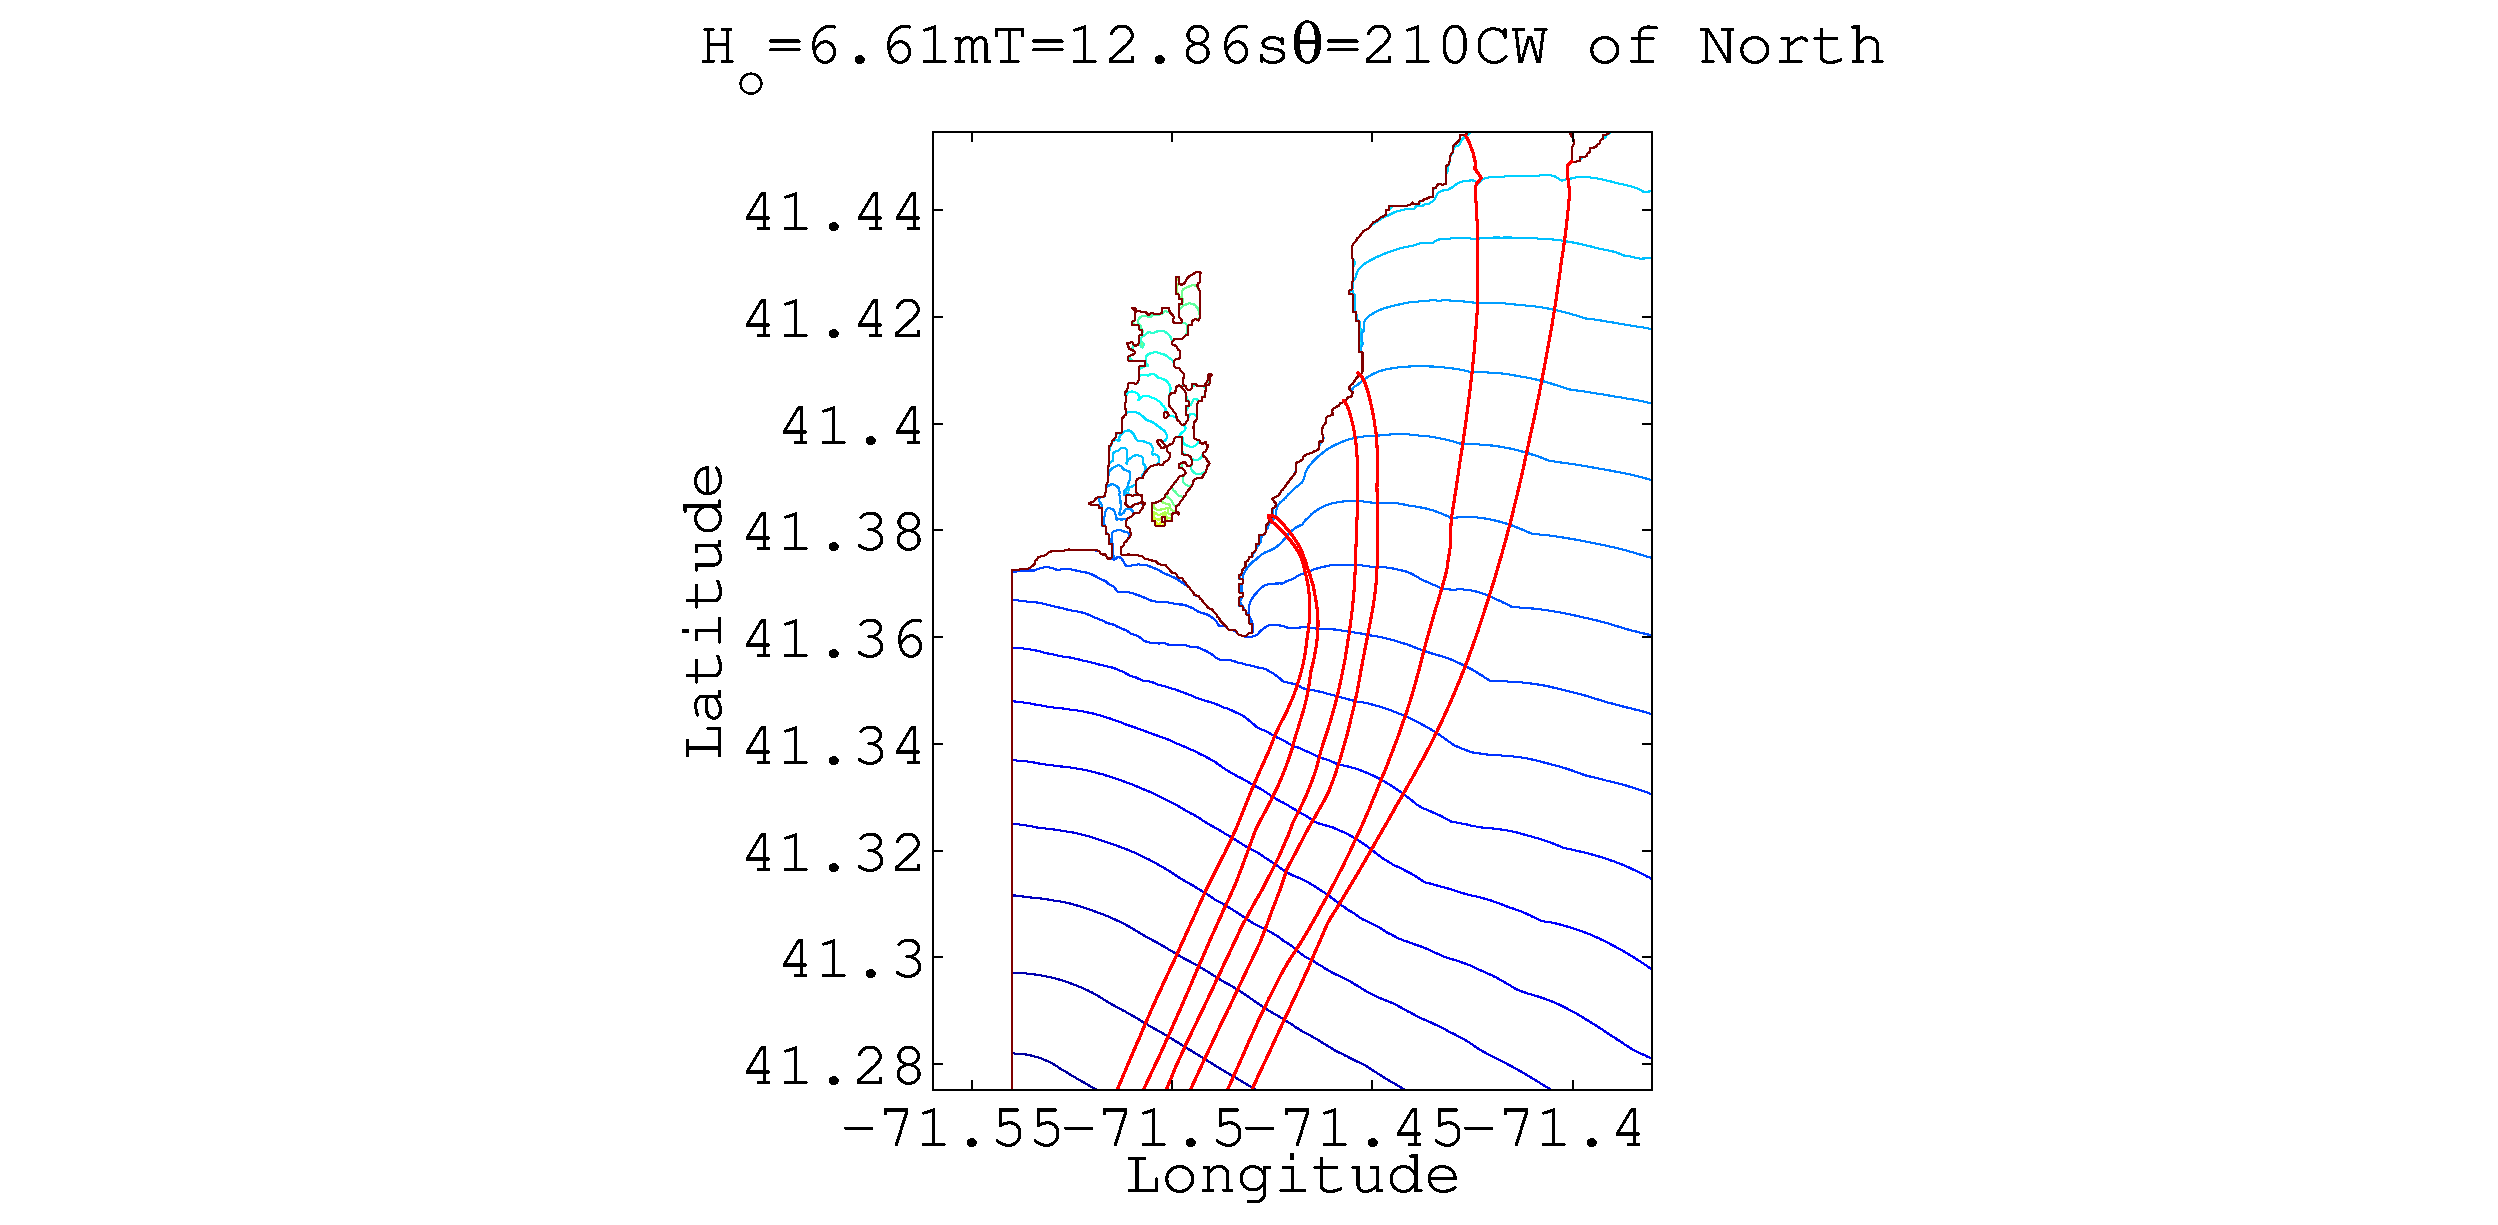
\includegraphics[width=1.0\textwidth]{./img/20y_210deg.pdf}
\caption{Breaking Wave Characteristics for 20 Year extreme wave at 210$^{\circ}$ angle of incidence}
\label{fig20y210deg}
\end{figure}

%\begin{figure}
%\centering
%\begin{minipage}{.33\textwidth}
%  \centering
%  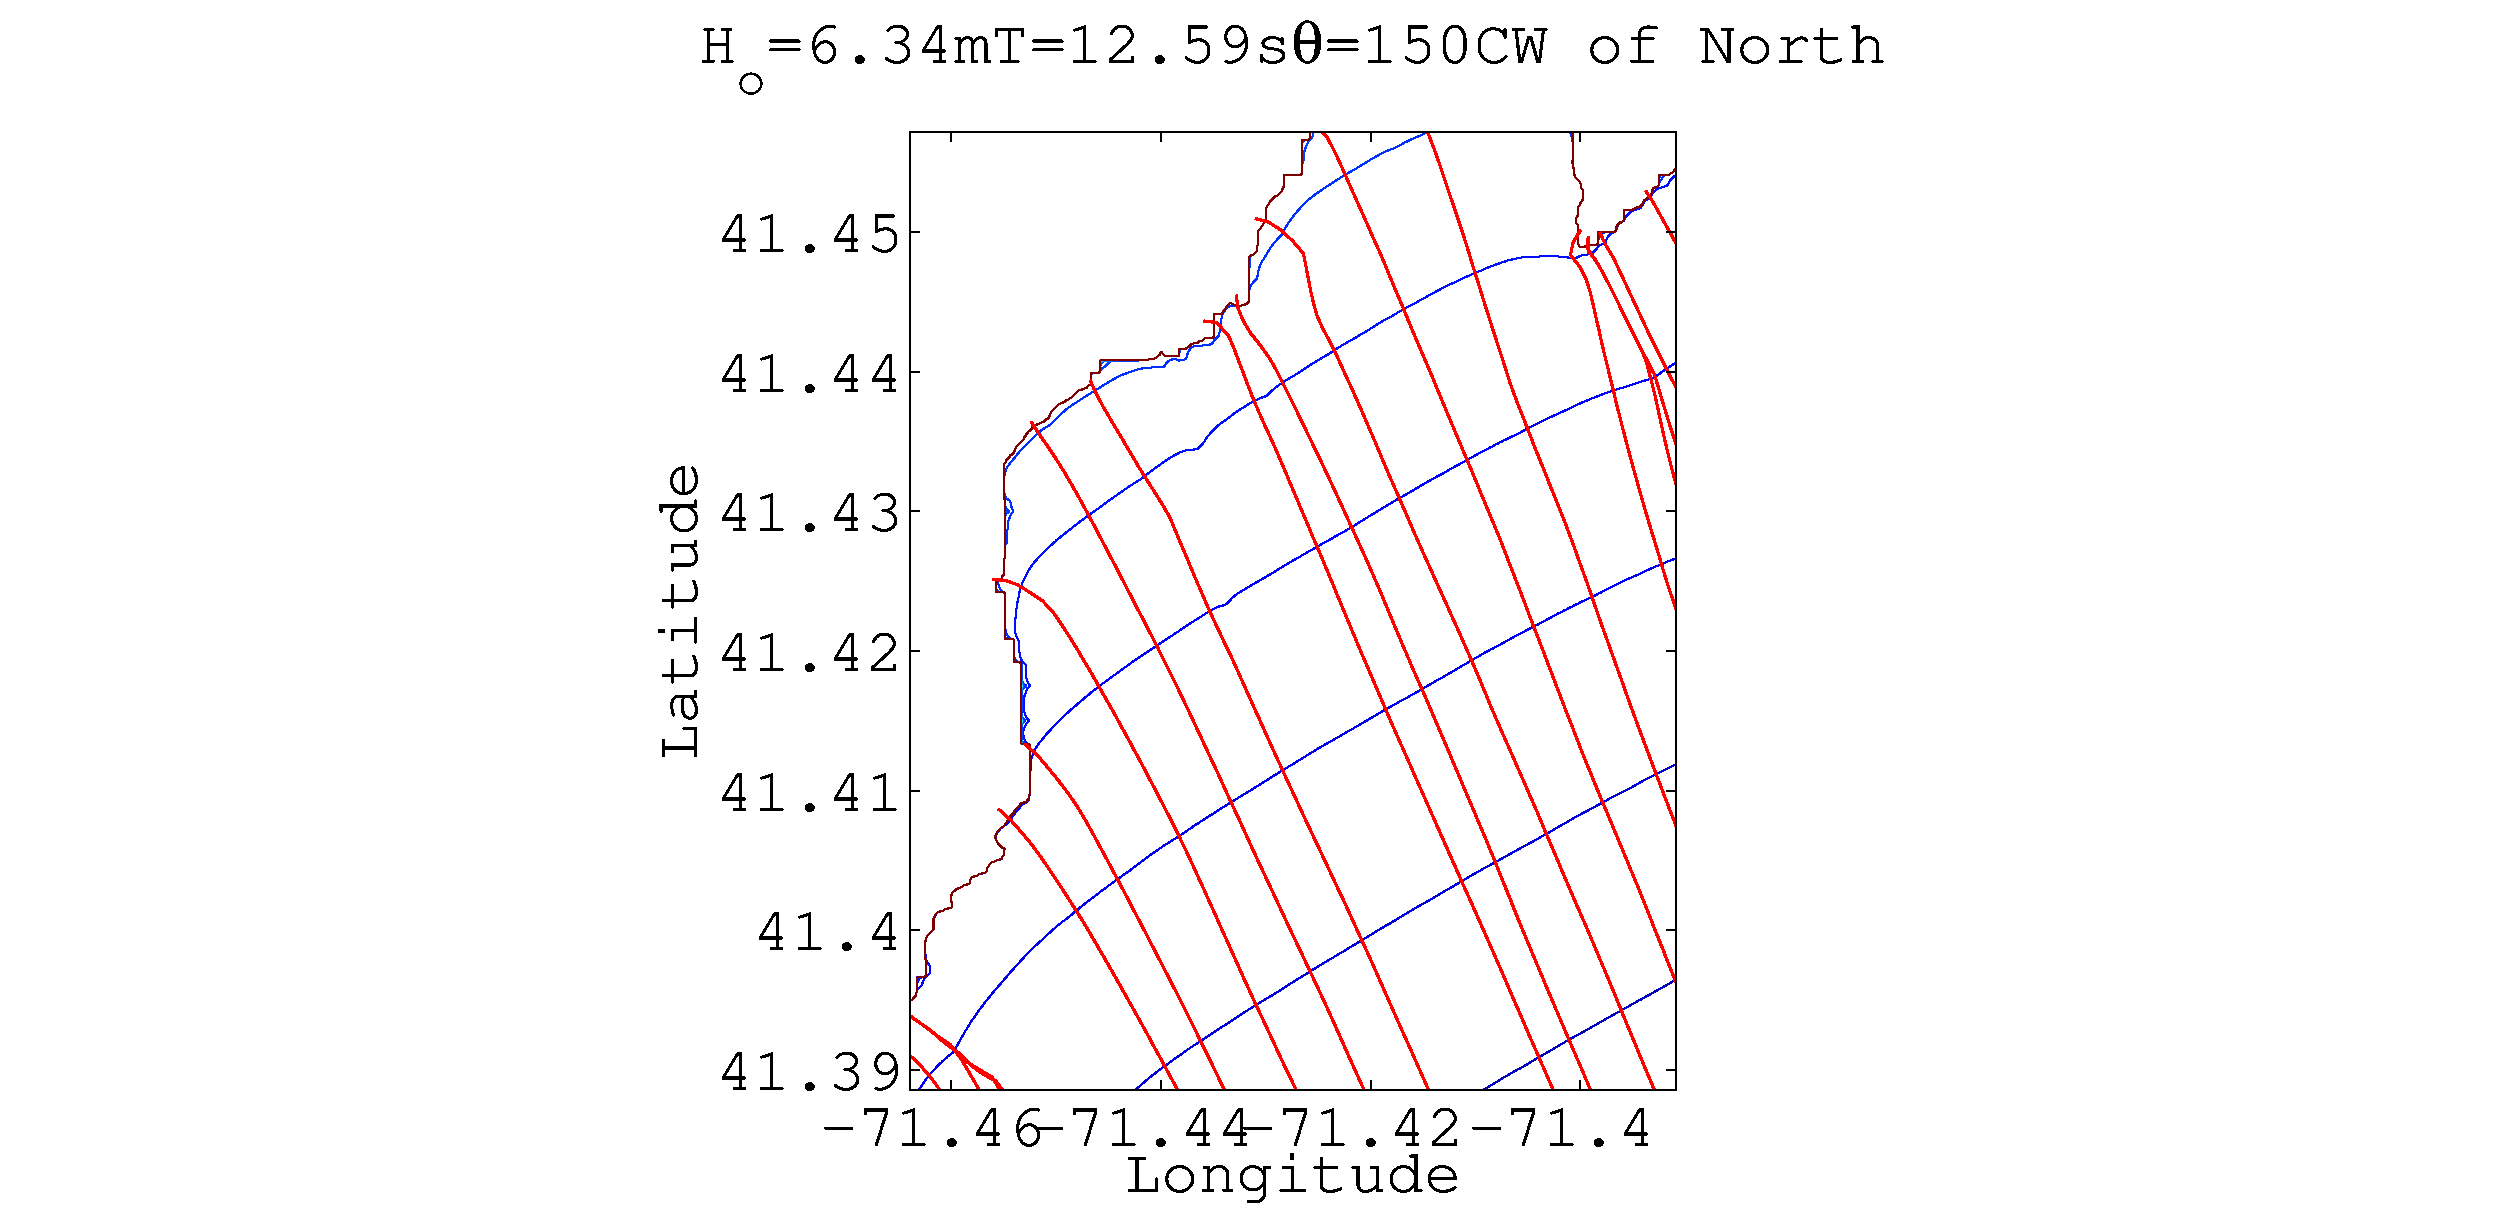
\includegraphics[width=1.2\textwidth]{./img/20y_150deg.eps}
%  \caption{20y, 150$^{\circ}$}
%  \label{fig:20y150deg}
%\end{minipage}%
%\begin{minipage}{.33\textwidth}
%  \centering
%  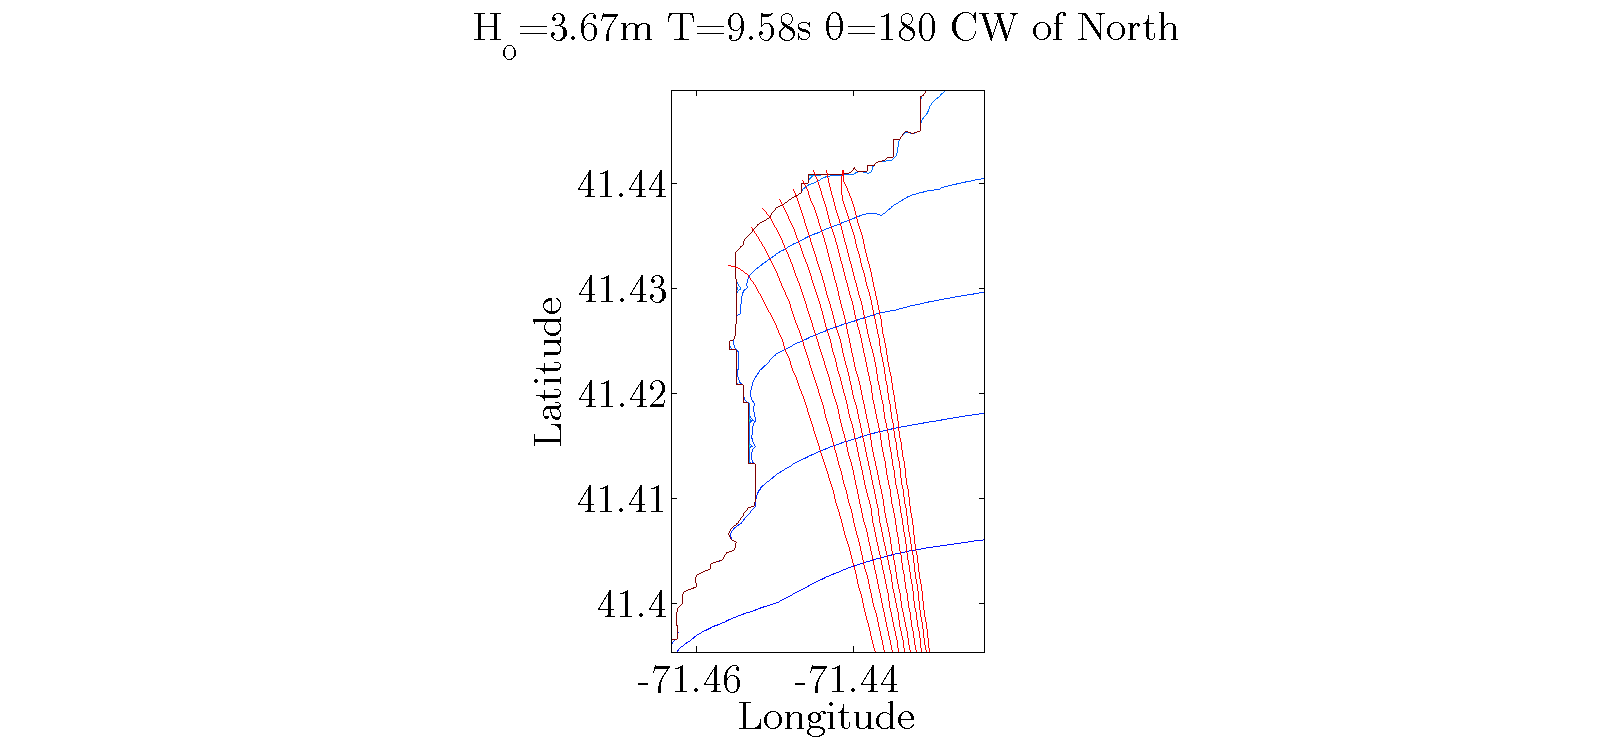
\includegraphics[width=1\linewidth]{./img/20y_180deg.eps}
%  \caption{20y, 180$^{\circ}$}
%  \label{fig:20y180deg}
%\end{minipage}
%\begin{minipage}{.33\textwidth}
%  \centering
%  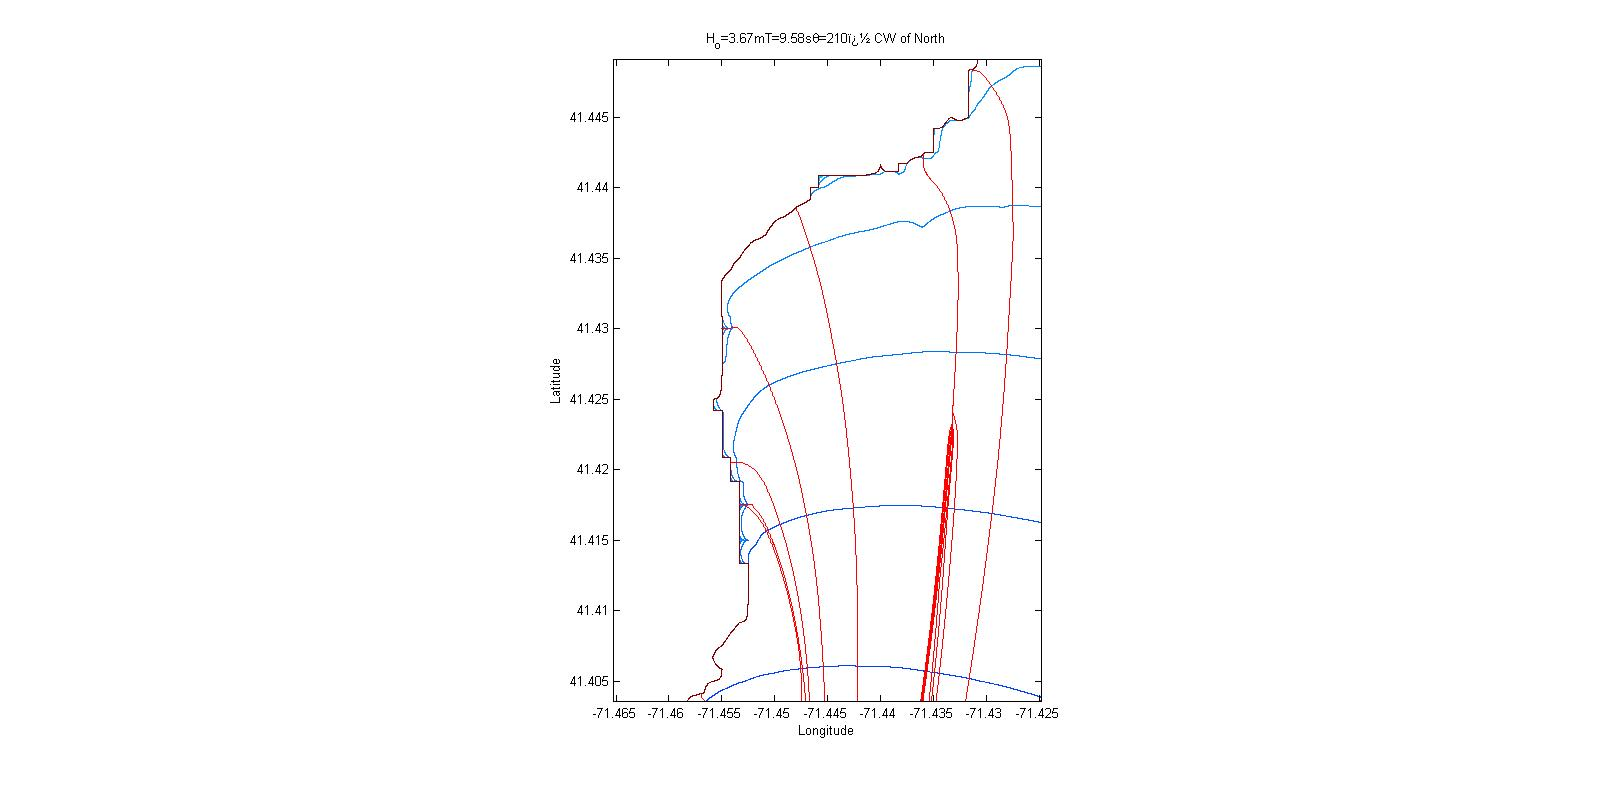
\includegraphics[width=1.2\linewidth]{./img/20y_210deg.eps}
%  \caption{20y, 210$^{\circ}$}
%  \label{fig:20y210deg}
%\end{minipage}
%\caption{20 Year Predicted Waves, H$_{o}$ = , T = }
%\label{fig:20y}
%\end{figure}

Seen below, the simulated wave rays for the 50 year extreme waves were very similar to their 20 year counterparts. Narragansett Beach de-focused the few rays that hit the beach, and the degree of de-focusing can be observed to increase as the angle of incidence approached 210$^{\circ}$.

\begin{figure}[H]
\centering
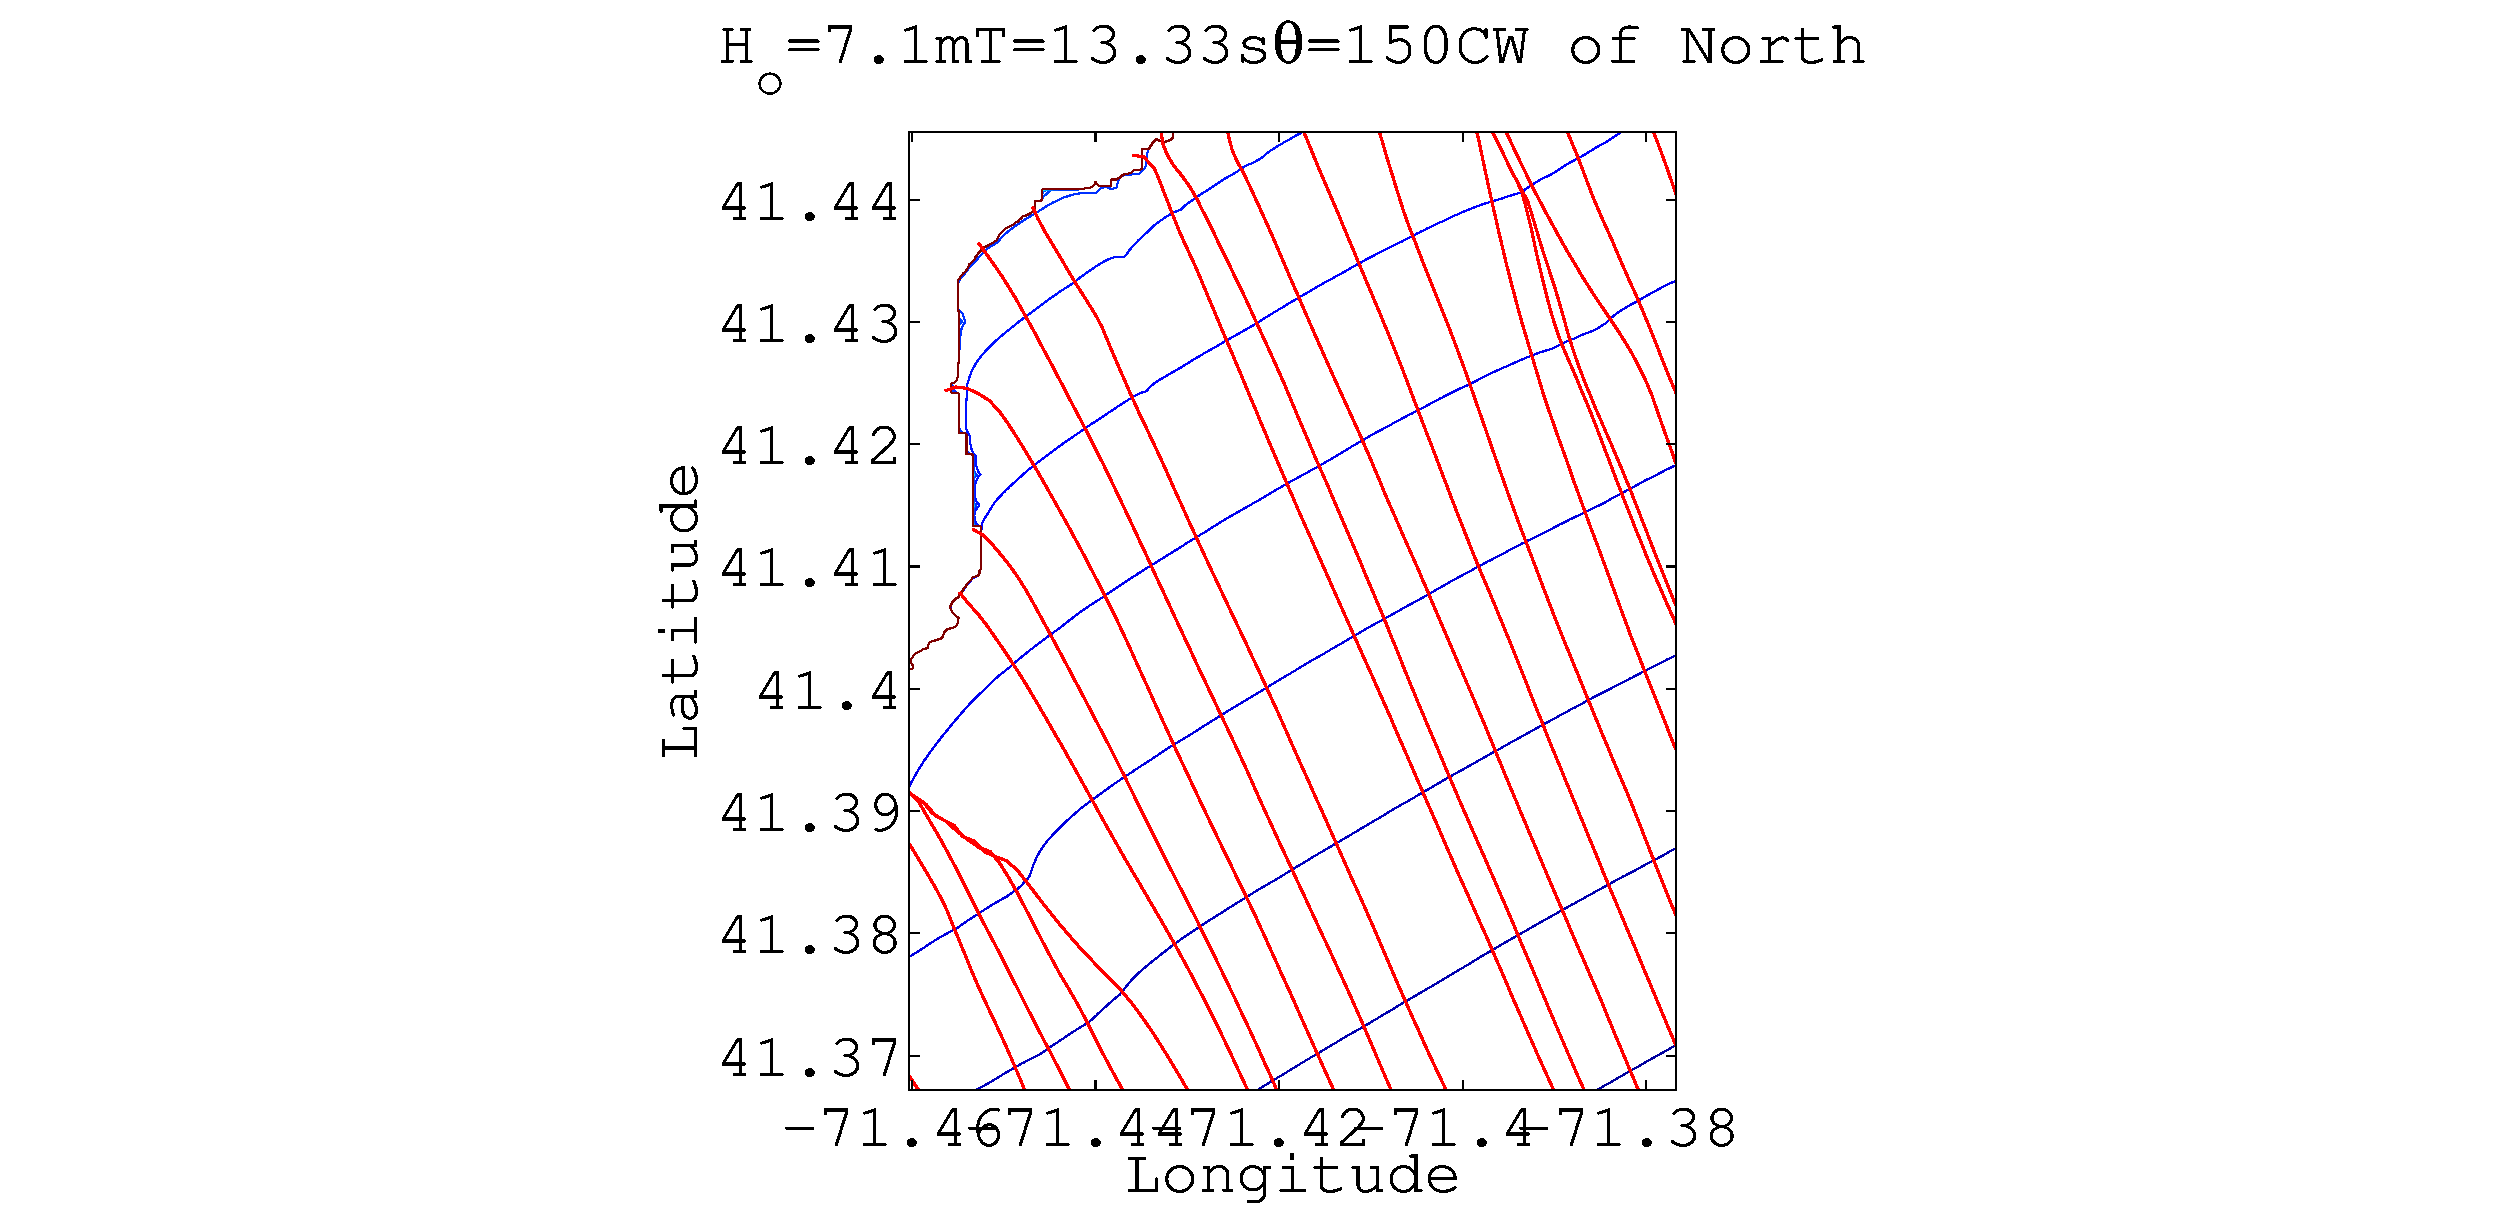
\includegraphics[width=1.0\textwidth]{./img/50y_150deg.pdf}
\caption{50y Predicted Wave Rays at 150$^{\circ}$ angle of incidence}
\label{fig:50y150deg}
\end{figure}

\begin{table}[H]
\centering
\begin{tabular}{cccccc}
Ray: & $K_{r}$ & $K_{s}$ & $H_{b}$ & $h_{b}$ & $\dfrac{H_{b}}{h_{b}}$ \\
\hline
1 & 1.0 & 0.1 & 6.2 & 8.6 & 0.7 \\
2 & 1.0 & 0.0 & 4.0 & 8.5 & 0.5 \\
\hline
\end{tabular}

\caption{Breaking Wave Characteristics for 50 Year extreme wave at 150$^{\circ}$ angle of incidence}
\label{tab:50y_150deg}
\end{table}

\begin{figure}[H]
\centering
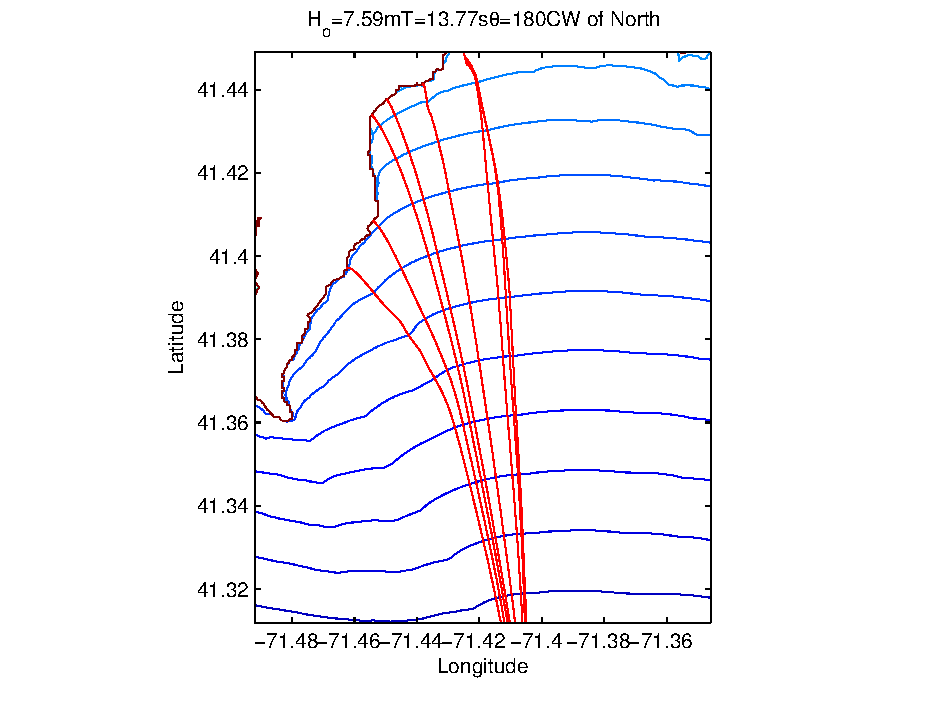
\includegraphics[width=0.6\textwidth]{./img/50y_180deg.pdf}
\caption{50y Predicted Wave Rays at 180$^{\circ}$ angle of incidence}
\label{fig:50y180deg}
\end{figure}

\begin{table}[H]
\centering
\begin{tabular}{cccccc}
Ray: & $K_{r}$ & $K_{s}$ & $H_{b}$ & $h_{b}$ & $\dfrac{H_{b}}{h_{b}}$ \\
\hline
1 & 1.0 & 0.1 & 6.8 & 9.2 & 0.7 \\
2 & 1.0 & 0.0 & 4.2 & 9.0 & 0.5 \\
\hline
\end{tabular}

\caption{Breaking Wave Characteristics for 50 Year extreme wave at 180$^{\circ}$ angle of incidence}
\label{tab:50y_180deg}
\end{table}

\begin{figure}[H]
\centering
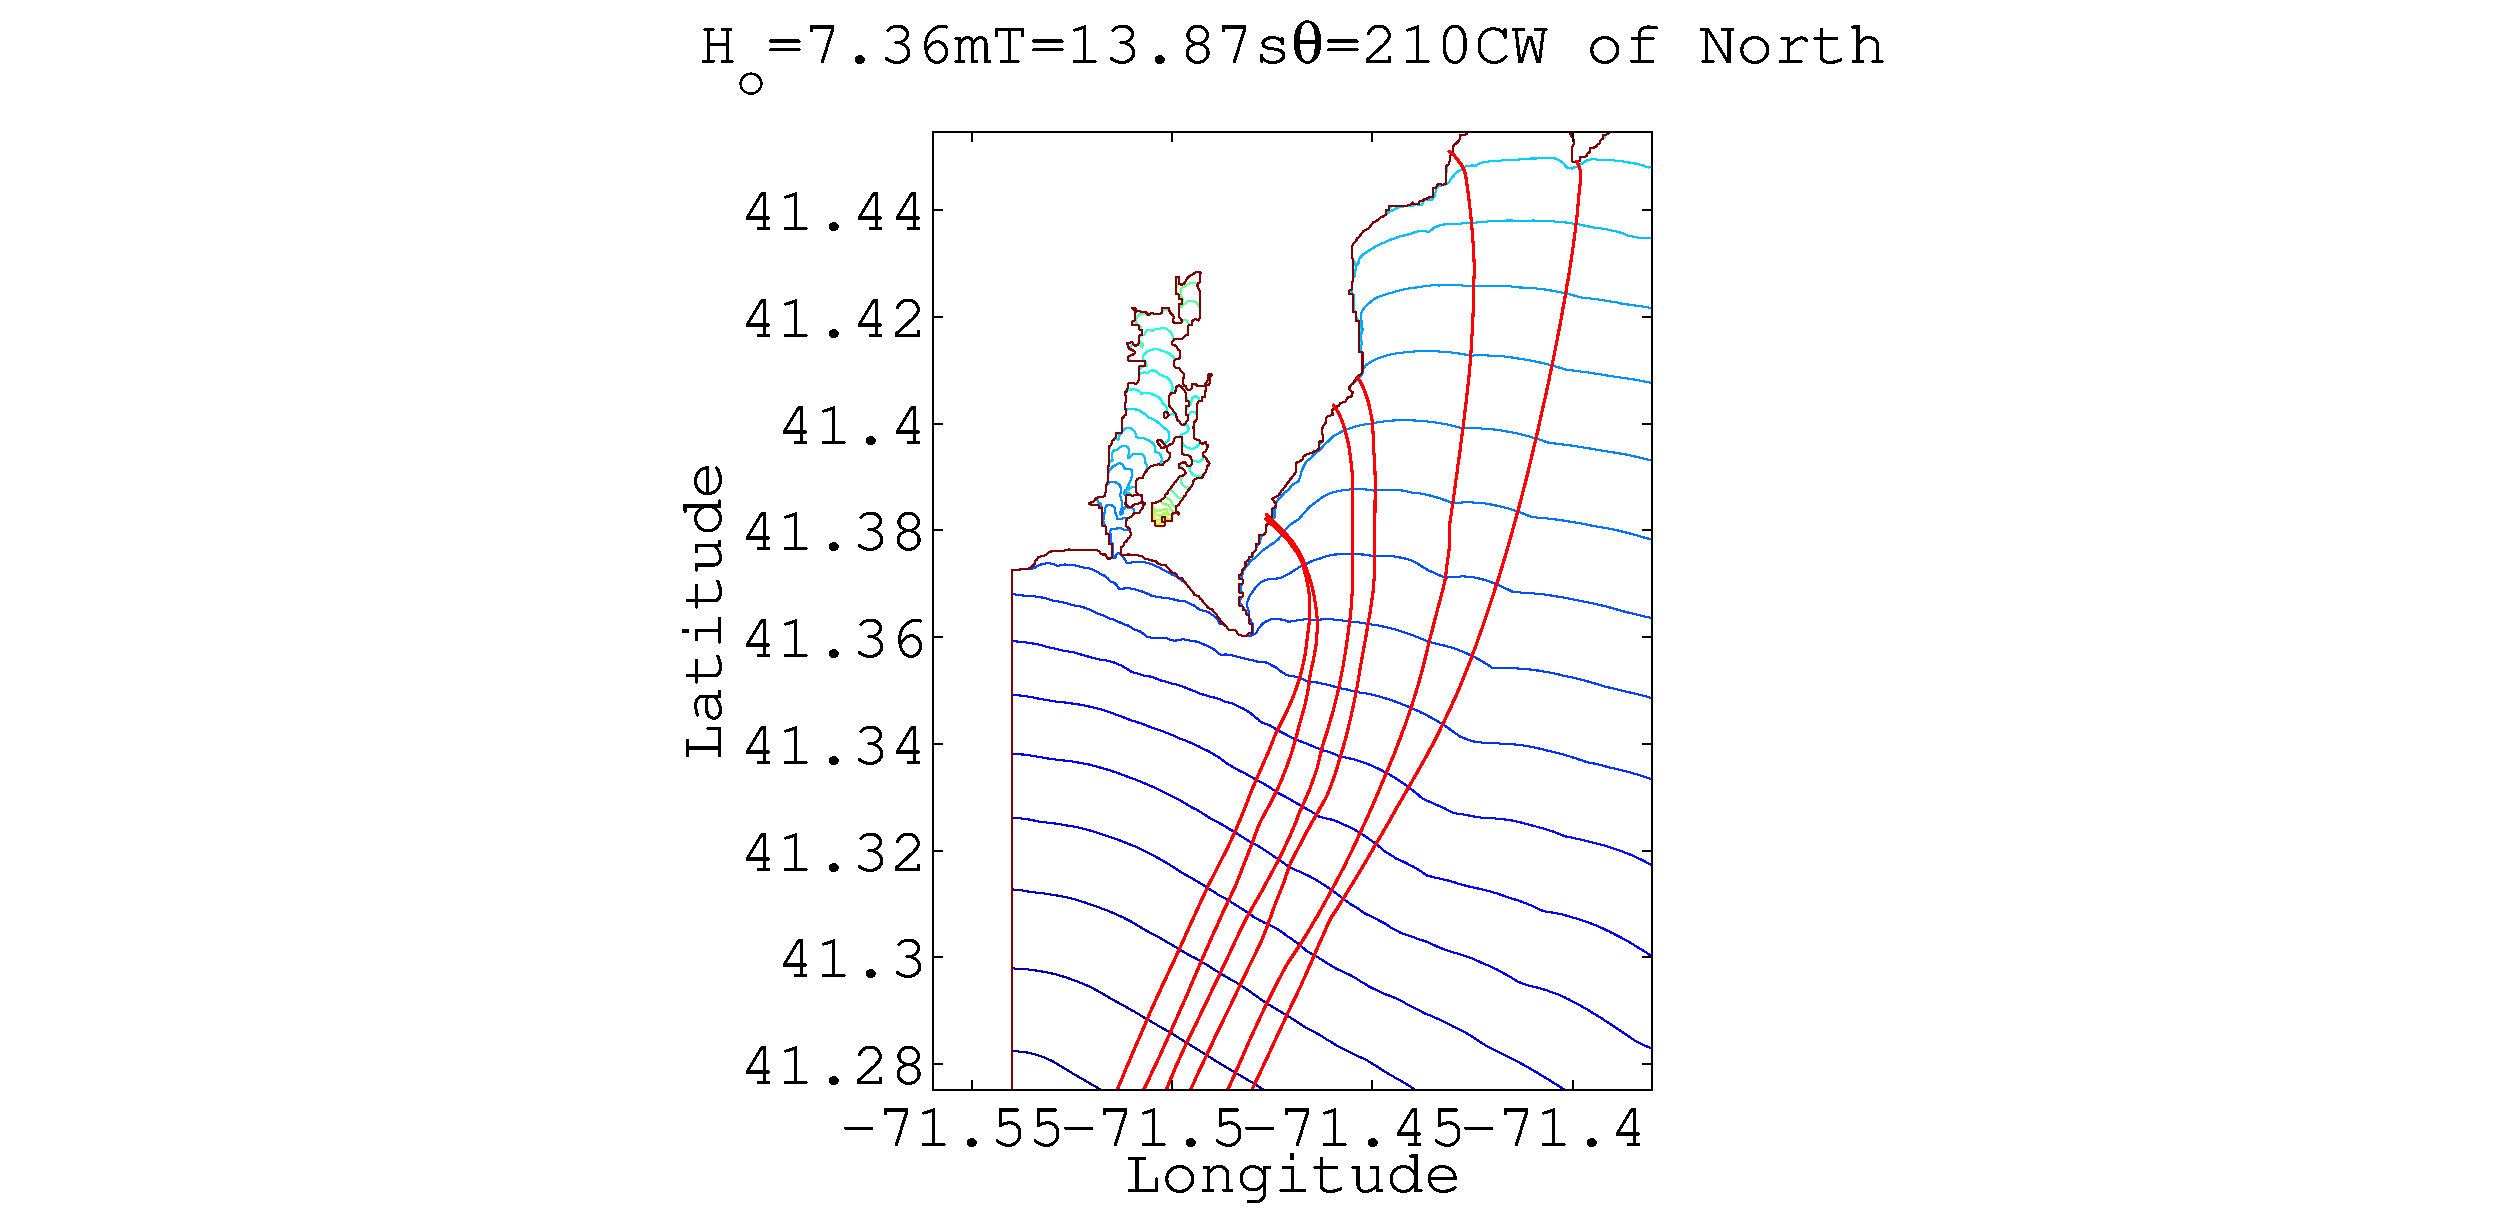
\includegraphics[width=1.0\textwidth]{./img/50y_210deg.pdf}
\caption{50y Predicted Wave Rays at 180$^{\circ}$ angle of incidence}
\label{fig:50y210deg}
\end{figure}

%Talkin bout sediment transport
Sediment transport 

%Talkin bout wave energy facility and location importance and such

%Talkin bout inclusion of diffraction model
Diffraction modeling would have influenced our 210$^{\circ}$ angle of incidence waves. Bloc

\section{Conclusion}
After manually evaluating the breaking wave characteristics, it indicated that the simulated wave rays would experience de-focusing. From the data in task 1, the simulated wave rays for the 50 year extreme showed similarity to their 20 year counterparts. Narragansett Beach also de-focused the rays that hit the beach. The degree of de-focusing can be observed to increase as the angle of incidence approaches 210$^{\circ}$ . Overall, using the supplied functions given, the wave ray analysis on Narragansett Beach under the conditions determined in task 1 proved that the simulated wave rays experienced de-focusing. 




